Previously, we have published results to show that different combinations of service providers and consumers led to significantly different service requirements within a MANET environment \cite{Macker2010}. This led to a prototype implementation of our Independent Network Discovery Interface (INDI) that addressed these concerns by providing three different profiles and flexible configuration parameters for applying bespoke timers and multicast distribution policies for these different mobile scenarios. We later discussed the adaptation of this implementation to work alongside mDNS to address the MANET architectural considerations and for maintaining full interoperability with existing mDNS enterprise deployments (e.g. Apple Bonjour, etc) \cite{Macker2011}. We also provided a functional empirical analysis of JmDNS, Bonjour and INDI mDNS when discovering single services on a LAN and showed that  INDI can have up to a twelvefold reduction in network messages over these existing protocols when discovering a single service on a LAN mainly because of the generic nature of the mDNS discovery scheme, described in the previous section.

By integrating INDI profiles on an existing mDNS infrastructure we aim to be able to offer robust service discovery mechanisms for use within a MANET and at the same time, remain interoperable with existing fixed infrastructure service discovery solutions, which will make it easier to integrate with existing applications. To achieve this, the underlying structure for an mDNS message needs to be understood as well as the the algorithm that mDNS employs to perform service discovery on a LAN.  By extracting these requirements, we will override the timers of these components and overlay modes in order for the same stack to operate using the new profiles and timers tuned for a MANET.  In the next section, we look at the structure mDNS in order to extract such requirements.

\subsection{Requirements from mDNS}
\label{sec:requirements}

An mDNS network comprises a number of mDNS responders (or Bonjour services), which implement the Multicast DNS specification for advertising and discovering mDNS services.  An mDNS responder uses link-local IP Multicast on UDP port 5353 for transmission and can optionally connect to a unicast DNS for service discovery anywhere in the world. mDNS uses DNS resource record data types provided in table \ref{table:resource:record}, which allow both host resources and services to be specified. Records can also use the DNS wildcard resource record (ANY) for matching  thereby enabling the ability to browse the network.  An mDNS formatted message contains a header, a question, answer, authority, and additional record sections, as shown in the ``mDNS Message'' section in Figure \ref{indi:fig:architecture}.   A given DNS record is capable of answering a DNS question if the record name matches the question name, the record \emph{rrtype} matches the question  \emph{qtype} (or the \emph{ qtype} is ``ANY'' (255) or the  \emph{rrtype} is ``CNAME'' (5)) and the record  \emph{ rrclass} matches the question  \emph{qclass} (unless the  \emph{qclass} is ``ANY'' (255)). 

%\vspace{-5pt}
\footnotesize
\begin{table}[h]
\caption{DNS resource records used by mDNS}
\label{table:resource:record}
\begin{center}
%\vspace{-12pt}
\begin{tabular}{| c | c  | p{7.5cm} |}

\hline \textbf{Resource Record} & \textbf{Abbr.} & \textbf{Description}\\

\hline Addressing & A &  Specify the IPV4 address of this host and are used to resolve IP addresses (see \cite{rfc1035}).\\

\hline

IPV6 Address & AAAA & Specify the IPV6 128-bit host address \cite{rfc1886}.\\
\hline

\hline
Text  & TXT & 

Specifies multiple strings of text, up to 255 characters long \cite{rfc1035}. \\

\hline
Wildcard  & ANY & 

Specifies a wildcard to match any number of labels in a name \cite{rfc4592}. \\
\hline

\end{tabular}
\end{center}
\end{table}
\normalsize


All mDNS packets contain an IP time to live (IP TTL) in the header for the hop-count limit (for link local, this should be 255 to indicate no forwarding).   An mDNS resource record also contains a RR TTL,  used to specify the  number of seconds for which the record may be cached.   The recommended TTL value for Multicast DNS with a host name as the resource record's name (e.g. A, AAAA, HINFO, etc.) or a host name contained within the resource  record's  \emph{rdata} (e.g. SRV, reverse mapping PTR record, etc.) is 120 minutes.   Other mDNS resource records have a TTL of 75 minutes.


Upon bootstrapping (start up, wake up from sleep, or that its network connectivity has changed), a mDNS responder performs two operations:  

\begin{itemize}
\item \textbf{Probing:}  three probes are sent onto the network, 1 second apart.  Probes query any of the resource records that desire to be unique on the local link are not already in use.  The primary use of this is to resolve a host's address record (A or AAAA) and identify address conflicts to map the unique host name to its unique IPv4 and/or IPv6 address.  Probe queries set the desired resource record name, class and query type to ``ANY'' (255), allowing a single question to be used in place of several questions. The probe queries also can contain service adverts that this mDNS responder is responsible for once the mDNS responder has announced itself on the network. In effect therefore, each message can contain a host record and/or several service records. 
\item   \textbf{Announcing:}  two announcements  are sent onto the network at 250 milliseconds intervals once probing has finished, regardless of operating role (i.e. server or client).  The announcer then sends the lists of service adverts it is responsible for once onto the network to advertise the list of services it has available to other users.  
\end{itemize}

The mDNS protocol first discovers abstract advertisements and then only resolves its endpoint when the client wishes to make use of it.  In the meantime, its address can change if a laptop moves IP address for example. Therefore, for client-side resolving of adverts, there are three resolvers that are used to query certain levels of service abstractions, as follows:

\begin{itemize}

 \item \textbf{Type Resolvers:}  that query the network for service types e.g. \_http.\_local.

\item \textbf{Service Resolvers:} that query for services of a given a specific name and type.
 
\item \textbf{Service Info Resolvers:} that resolve the address for a service, given its name.
\end{itemize}

Each resolver queries the network three times at 225 millisecond intervals.  A client then goes into probing mode, making three 1 second interval queries and then onto the announcer for two further queries.  After announcing has finished, the client can be considered initialized and can starting resolving services.     The client attaches itself as a listener to asynchronously discover services through notification.  Two service resolvers are set up by JmDNS: the first listens for any occurrences of the service name, converted to lower case, and the second for the name provided as is.  

Therefore, from a protocol perspective, there are five entities that control the algorithm that mDNS uses to exchange messages at particular intervals between mDNS responders.  These entities form the foundation for the resulting architecture, design and implementation of INDI mDNS, which is described in the following sections. 


\subsection{Architecture and Design}
\label{sec:architecture-design}

In the previous section, the mDNS requirements have been provided.  Through the aforementioned previous experiments \cite{Macker2010} covering several hundred simulations across a broad range of service discovery schemes (reactive and proactive), we found that the following parameters were required in order to meet the design needs for the range of applications we are interested in:

\begin{itemize}

\item  \textbf{AdvertLifetime:} lifetime (TTL) that the service. For JmDNS, this is fixed but in INDI, this can be adjusted for the particular application. 
\item  \textbf{ReadvertisementInterval:} interval that providers proactively send out service advertisements onto the network e.g. a service provider can periodically send out its advertisements every 5 seconds.  
\item  \textbf{NumReadvertisements:}  number of times to readvertise the service or you can set this value to -1, which means advertise forever.
\item  \textbf{ClientQueryIntervals:}   are the times at which a client sends out queries for services onto the network and is 
specified for flexibility using a \emph{timeouts} array of absolute millisecond times for sending out a query, e.g. 0, 100, 200, 400, 800, would send queries at 0, 100, 200, 400 and 800 milliseconds.
\item  \textbf{ServiceCancelInterval:}  specifies the interval at which to send proactive service cancel notifications. A cancell message can be used to notify distributed mDNS peers that an advert should be deleted.
\item  \textbf{NumServiceCancelMessages:}  number of times to send proactive service cancelled packets.
\item \textbf{Port:}  port to send messages (default is mDNS, 5353)
\item \textbf{Send Wait Interval (OppCache):} offset interval before switching to reactive mode. This enables a wait time for a client to listen for proactive advertisements before entering into a query phase.

\end{itemize}

Collectively, these parameters can be used to implement a number of different modes and message exchanges.  Parameters can be set to approximate mDNS behavior using a combination of reactive and proactive timer setting but cannot be configured to replicate mDNS exactly.  However, for a MANET, we can group combinations of these parameters to form three broad INDI modes (setting profiles) for simpler use:  \textbf{Reactive:} where the consumer dispatches a service request using a query and providers respond with a service advert (i.e. the Responder in Figure  \ref{indi:fig:architecture}); \textbf{Proactive:} where the providers perform a service push by periodically sending out their service adverts using multicast;  and \textbf{Opportunistic Caching:}  is based on the concept that if a consumer queries for a service, other consumers may be interested in that service i.e. we opportunistically cache for future use.  The three profiles therefore need to be layered onto the entities described in Section \ref{sec:requirements} to form the basis for the implementation of INDI, whilst retaining the underlying interoperability of mDNS messages. 

\begin{figure}
%\vspace{00pt}
\centering
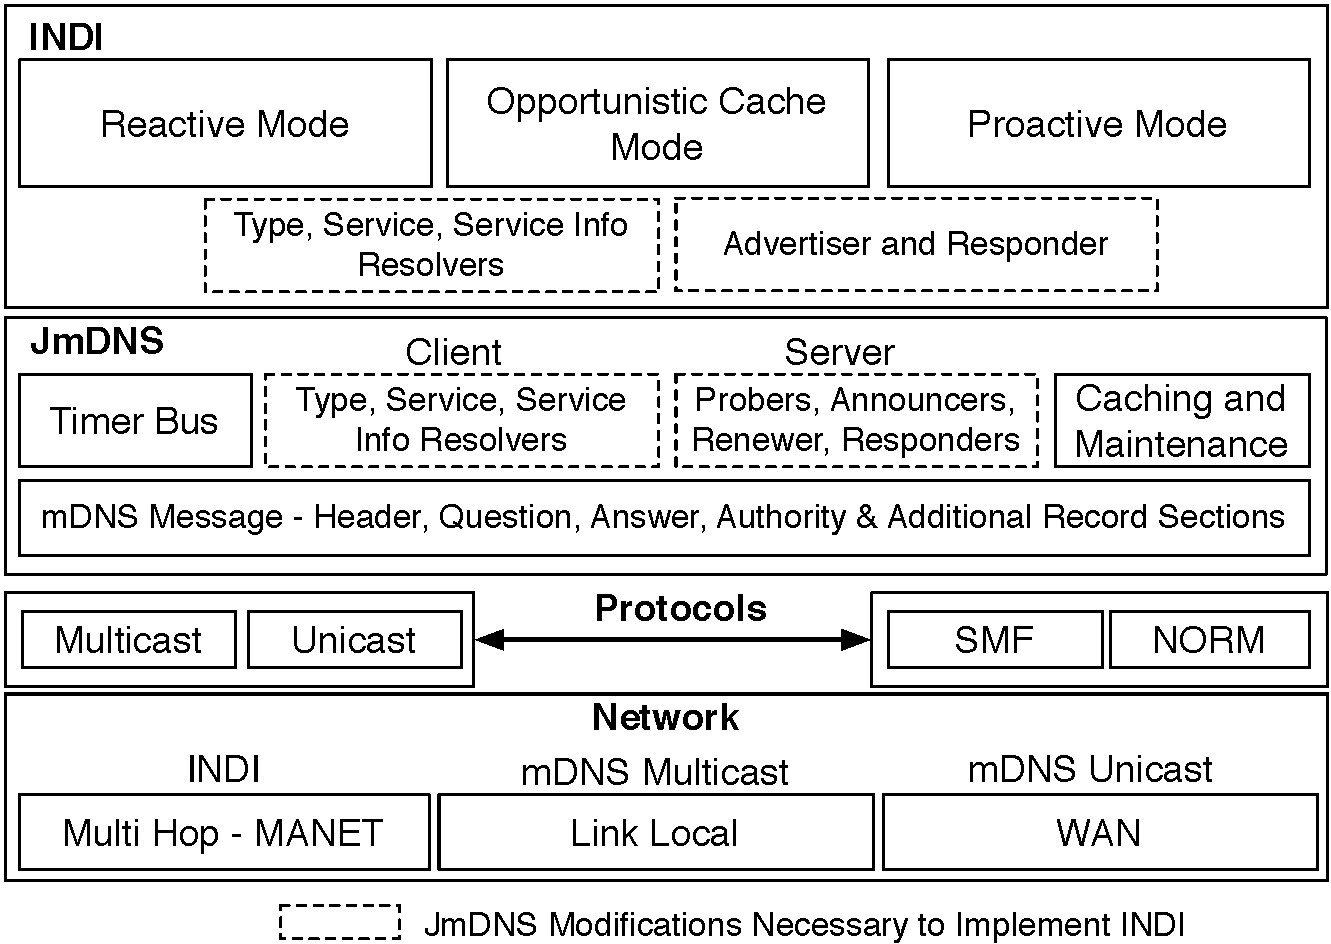
\includegraphics[scale=0.55]{INDIArchitecture.pdf}
%\vspace{-8pt}
\caption{INDI Architecture} \label{indi:fig:architecture}
%\vspace{-20pt}
\end{figure}

Figure  \ref{indi:fig:architecture} shows the resulting architecture for INDI taking into consideration the INDI design specification and the mDNS entities used to implement the mDNS functionality.  This architecture shows a schematic for the layering of the INDI design profiles: reactive; opportunistic cache; and proactive, onto the existing advertiser and responder, type, service, info resolvers.     It can be seen that for the client side, JmDNS entities are similar to INDI, the major differences being in the number of resolvers deployed and the timings of retries to support the INDI design configurations.  However, the server side protocol is significantly different with INDI only requiring advertising and responding roles compared with JmDNS that has probe, announce, responder and renew roles.  The advertising role in INDI is a simplification of the probe, announce and renew roles in mDNS.

The rest of the software architecture mimics JmDNS as illustrated in Figure  \ref{indi:fig:architecture}. Once packaged by the different entities, the message format can use the same messaging serializer and on-the-wire format to remain compatible with DNS.  INDI therefore should be 100\% JmDNS/mDNS, AVAHI and Bonjour interoperable.   

For the networking level, the conventional deployment of JmDNS and INDI differs considerably. Whilst on a static infrastructure LAN, the protocols being used would be standard multicast and unicast, on a MANET, these underlying protocols would generally be replaced by more flexible and adaptive protocols to cope with the changing infrastructure more effectively. An issue that impacts critically here, is the link-local scoping of  mDNS that forms part of the specification.   Therefore, since mDNS is intended for link local operation and there are presently no de facto standards or accepted addressing practices for extensions to site-local or multi-hop ad hoc network operation, we also support ``proof-of-concept'' multi-hop operation through a SMF (Simple Multicast Forwarding) \cite{macker2004simplified} plugin, which forwards mDNS messages for site-scoped  areas, where mobile ad hoc routing may require highly dynamic edge routing.  This solution provides an administratively scoped multi-hop capability versus the more typical single network hop IP link-local multicast capability used by many deployed service discovery approaches.  

These same types of optimized flooding algorithms are also available in many ad hoc routing control planes and existing research has demonstrated the ability to encapsulate service discovery messaging within the control plane mechanism \cite{li-lightweight}. We do not suggest a particular approach to the message forwarding here, as there are many valid options and INDI supports standard IP multicast traffic that can also be adapted for middleware encapsulation.  Rather, we focus on examining the use of such techniques, whether encapsulated or not, to enable the potential for more robust distributed querying, response, and proactive notification.

%For example, previously we have used the Essential Connected Dominating Set (ECDS) algorithm \cite{Macker:2007:SMFCDS} in deployment for multicast routing.  Here, the backbone is calculated in a distributed manner based on localized neighbor information and the selected CDS algorithm.  Selected nodes rebroadcast all non-duplicate multicast packets providing network wide flooding for all multicast traffic.  

\subsection{Implementation}
\label{sec:implementation}

We have been working closely with the JmDNS community \cite{jmdns} provide a pluggable architecture in JmDNS for INDI to be able to provide different functionality for the mDNS entities described in Section \ref{sec:requirements} for overlaying INDI profiles (see Section \ref{sec:architecture-design}).  The JmDNS \cite{jmdns} authors provided customization of the Java timing interfaces to the JmDNS entities for our use to integrate custom tasks for layering INDI modes, which is shown in Figure  \ref{indi:fig:architecture}.   
    
For the entities, we replace the \emph{Prober}, \emph{Announcer} and \emph{Renew} tasks with an Advertiser class, which performs the proactive advertisements as and when they are required.  A and AAAA records are not included in the advertisements because in a MANET, other address mechanisms are in place to avoid potential conflicts here.  INDI includes a modified \emph{Responder} for replying to tasks, which switches between unicast and multicast depending on the mode we are working within i.e. for Opportunistic cache and Proactive modes the responder replies with a multicast message and in Reactive, it replies with a unicast message.

On the client side, the type, service and service info resolvers resemble the JmDNS variants with three main differences.   INDI resolvers always check the cache before sending out queries to the network.   Secondly, the sequence of solicitations for resolving queries is different.  A user can specify any sequence they choose in INDI so this is a user preference depending on the application.  Third, the responses from the resolver are far more aggressively propagated to the resolvers in INDI.  This results in less queries being sent because as soon as a reply to a query has been received, the resolver quits operation.     
 
There are other housekeeping classes that differ in the INDI implementation.    We have the INDI \emph{Canceller} that can be customized to send out packets onto the network at whatever interval a user chooses or can be turned off to act in a completely passive manner and allow the TTL to expire the advertisement.  For example, for the experiments in Section \ref{sec:methodology}, we do not send any cancel messages onto the network because the TTL is so short we do not need further proactive behavior from the other components.  Instead, we use the INDI \emph{RecordReaper}, which is far more aggressive than the JmDNS counterpart.  Reaper intervals can be specified in the configuration depending on the frequency one would like to check the cache and expunge out of date advertisements.  For JmDNS, this is generally performed to coincide with other requests but in INDI one can program it to check at the millisecond level.   For the experiment described in  Section \ref{sec:methodology}, we use a reaper interval of 500 milliseconds. 

INDI provides a profile structure that build up layers according to the profiles defined through combinations of the core parameters defined in the previous section.  The Java class \emph{Profile} provides rudimentary defaults for all modes.   Client query intervals (for the resolver implementations) are set to trigger at 0, 100, 200, 400, 800 and 1600 milliseconds, respectively. The default TTL is set to the the mDNS specification recommended value of 2 hours and the readvertisement interval is set to half that value, also as recommended in the specification.  These defaults are inherited  by the \emph{Reactive} class, which exhibits the most similar behavior to mDNS.   The \emph{Opportunistic Cache}  profile also inherits the same behavior as \emph{Reactive} but it differs in that it responds to queries using multicast so that other INDI nodes can opportunistically cache the results. It also differs in that it does not proactively request a service until it first checks its cache to see if one that matches has already been cached (by using the Send Wait Interval).

The \emph{Proactive} profile, on the other hand, is significantly different.  First, the TTL value is generally a lot shorter.   For the experiments, we describe in Section \ref{sec:methodology}, we use a TTL of 2 seconds and a readvertisement interval of 1 second.   Second, the endpoints are always included in the proactive announcements because the readvertisement rate is so high that the endpoints are constantly refreshed anyway. Therefore the resolvers generally are never need to send out resolver queries, so the sequence of resolver timeouts is changed to make sure the cache is checked before any resolving sequence takes place.  
  
